\begin{frame}{Gradient Boosting -- Functionality}

\footnotesize

\maketag{supervised}
\maketag{NON-PARAMETRIC}
\maketag{BLACK-BOX}
\maketag{FEATURE SELECTION}

\medskip

\highlight{General idea}

\begin{itemize}
  \item \textbf{Gradient boosting (GB)} is an \textbf{ensemble} method that 
  constructs a strong learner from weak base learners (frequently, CART).
  \item As opposed to \textbf{bagging}, however, base learners are assembled in a 
  \textbf{sequential, stage-wise} manner: in each iteration, GB improves the 
  current model by adding a new component that minimizes empirical risk.
  \item Each base learner is fitted to the current \textbf{point-wise residuals} 
  \\ $\rightarrow$ One boosting iteration $\widehat{=}$ one approximate 
  \textbf{gradient step in function space}
  \item The final model is a weighted sum of base learners $b(\xv, \thetam)$ 
  with weights $\betam$.
\end{itemize}

\medskip

\highlight{Hypothesis space} ~~
$\Hspace = \left\{ \fx: \fx = \sum_{m = 1}^M \betam b(\xv, \thetam) \right\}$

\begin{minipage}{0.5\textwidth}
  
\includegraphics[width=0.95\textwidth]{figure/gb-2d}
\end{minipage}%
\begin{minipage}{0.5\textwidth}
  % FIGURE SOURCE: http://arogozhnikov.github.io/2016/06/24/gradient_boosting_explained.html
  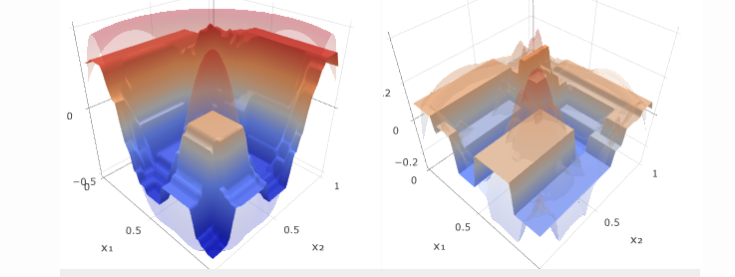
\includegraphics[width=\textwidth]{figure/gb-3d}
\end{minipage}

\tiny 
\textit{Left}: univariate gradient boosting, \textit{right}: bivariate gradient
boosting (1: target function (transparent) \& current ensemble, 2: residual 
(transparent) \& next 
tree, both taken from 
\href{http://arogozhnikov.github.io/2016/06/24/gradient_boosting_explained.html}{www.arogozhnikov.github.io})

\end{frame}

% ------------------------------------------------------------------------------

\begin{frame}{Gradient Boosting -- Functionality}

\footnotesize

\highlight{Empirical risk}

\begin{itemize}
  \item \textbf{Outer loss:} Loss used to compute pseudo-residuals -- how large 
  is the error of the current model fit? \\
  $\rightarrow$ Arbitrary \textbf{differentiable} loss function
  \item \textbf{Inner loss:} Loss used to fit next base learner component to 
  current pseudo-residuals \\
  $\rightarrow$ Typically, \textbf{quadratic loss} (desirable 
  optimization properties)
\end{itemize}

\medskip

\highlight{Optimization} ~~ \textbf{Functional gradient descent} for outer 
optimization loop, procedure for inner one depending on inner loss

\medskip

\highlight{Hyperparameters}

\begin{itemize}
  \item \textbf{Ensemble size}, i.e., number of base learners
  \item \textbf{Learning rate}, i.e., impact of single base learner
  \item \textbf{Complexity} of base learners (depending on type used)
\end{itemize}

\medskip

% \highlight{Runtime behavior} ~~ $\mathcal{O}(M \cdot n \cdot p)$ 
% for $M$ base learners, $n$ observations and $p$ features

\end{frame}

% ------------------------------------------------------------------------------

\begin{frame}{Gradient Boosting -- Pro's \& Con's}

\footnotesize

\begin{columns}[onlytextwidth]
  \begin{column}{0.5\textwidth}
    \highlight{Advantages}
    \footnotesize
    \begin{itemize}
      \positem Powerful \textbf{off-the-shelf} method for supercharging weak 
      learners' performance
      \positem Translation of most of \textbf{base learners'} advantages 
      (e.g., for tree boosting: inherent 
      variable selection, handling of missing data)
      \positem High predictive \textbf{accuracy} that is hard to outperform
      \positem High \textbf{flexibility} (custom loss functions, many tuning 
      options) 
      \positem Applicable to \textbf{unbalanced} data
    \end{itemize}
  \end{column}
  \begin{column}{0.5\textwidth}
    \highlight{Disadvantages}
    \footnotesize
    \begin{itemize}
      \negitem Hardly \textbf{interpretable} -- black-box method
      \negitem Hard to \textbf{visualize}
      \negitem Prone to \textbf{overfitting}
      \negitem Sensitive to \textbf{outliers}
      \negitem Hard to \textbf{tune} (high sensitivity to variations in 
      hyperparameter values)
      \negitem Rather \textbf{slow} in training
      \negitem Hard to \textbf{parallelize}
    \end{itemize}
  \end{column}
\end{columns}

\vfill

\small

\conclbox{High-performing predictor, but rather delicate to handle}

\end{frame}

% ------------------------------------------------------------------------------

\begin{frame}{Gradient Boosting -- Practical hints}

\footnotesize

\highlight{XGBoost (extreme gradient boosting)} 

Fast, efficient implementation of gradient-boosted decision trees that has
become \textbf{state of the art} for many machine learning problems \\
$\rightarrow$ Clever modeling techniques + computational speed \\

\medskip

\highlight{Stochastic gradient boosting (SGB)}

Faster, approximate version of GB that performs each iteration only on 
\textbf{random subset} of the data \\

\medskip

\highlight{Implementation}

\begin{itemize}
  \item \textbf{R:} \code{mlr3} learners \code{LearnerClassifXgboost} / 
  \code{LearnerXgboost}, calling \code{xgboost::xgb.train()}
  \item \textbf{Python:} \code{GradientBoostingClassifier} / 
  \code{GradientBoostingRegressor} from package \code{scikit-learn}, 
  \code{XGBClassifier} / \code{XGBRegressor} from package \code{xgboost}
\end{itemize}

\medskip

\highlight{Tuning}
\begin{itemize}
  \item Overall \textbf{limited tunability}
  \item Number of split candidates often more impactful than number of trees
\end{itemize}

\end{frame}